\documentclass[conference]{IEEEtran}
\IEEEoverridecommandlockouts
% The preceding line is only needed to identify funding in the first footnote. If that is unneeded, please comment it out.
\usepackage{cite}
\usepackage{amsmath,amssymb,amsfonts}
\usepackage{algorithmic}
\usepackage{graphicx}
\usepackage{textcomp}
\usepackage{xcolor}
\usepackage{hyperref}
\usepackage{nohyperref}
\newcommand{\BibTeX}{\textrm{B \kern -.05em \textsc{i \kern -.025em b} \kern -.08em
T \kern -.1667em \lower .7ex \hbox{E} \kern -.125emX}}
\begin{document}

    \title{Mining Massive Data Sets Midterm Report}

    \author{
        \IEEEauthorblockN{1\textsuperscript{st} 522H0036 - Luong Canh Phong}
        \IEEEauthorblockA{
            \textit{Faculty of Information Technology} \\
            \textit{Ton Duc Thang University}\\
            Ho Chi Minh City, Vietnam \\
            522H0036@student.tdtu.edu.com
        }
        \and
        \IEEEauthorblockN{2\textsuperscript{nd} 522H0092 - Cao Nguyen Thai Thuan}
        \IEEEauthorblockA{
            \textit{Faculty of Information Technology} \\
            \textit{Ton Duc Thang University}\\ \
            Ho Chi Minh City, Vietnam \\
            522H0092@student.tdtu.edu.com
        }
        \and
        \IEEEauthorblockN{3\textsuperscript{rd} 522H0075 - Tang Minh Thien An}
        \IEEEauthorblockA{
            \textit{Faculty of Information Technology} \\
            \textit{Ton Duc Thang University}\\
            Ho Chi Minh City, Vietnam \\
            522H0075@student.tdtu.edu.com
        }
        \and
        \IEEEauthorblockN{4\textsuperscript{th} 522H0167 - Truong Tri Phong}
        \IEEEauthorblockA{
            \textit{Faculty of Information Technology} \\
            \textit{Ton Duc Thang University}\\
            Ho Chi Minh City, Vietnam \\
            522H0167@student.tdtu.edu.com
        }
        \and
        \IEEEauthorblockN{5\textsuperscript{th} Instructor: Nguyen Thanh An}
        \IEEEauthorblockA{
            \textit{Faculty of Information Technology} \\
            \textit{Ton Duc Thang University}\\
            Ho Chi Minh City, Vietnam \\
            nguyenthanhan@tdtu.edu.com
        }
    }

    \maketitle

    \begin{abstract}
        This project implements and evaluates key techniques in mining massive datasets.
        It covers hierarchical agglomerative clustering of string shingles using Jaccard distance; PySpark-based linear regression for gold price prediction;
        CUR decomposition for feature dimensionality reduction on gold price data; and PageRank analysis of the \texttt{it.tdtu.edu.vn} web graph using PySpark.
        The work demonstrates practical applications and provides insights into processing large-scale data.
    \end{abstract}


    \section{Introduction}
    \label{sec:introduction}
    The increasing volume of data requires efficient mining techniques.
    This project implements and analyzes four core algorithms: (1) hierarchical agglomerative clustering for non-Euclidean text data, using 4-shingles and Jaccard distance on alphabetical strings; (2) PySpark-based linear regression to predict Vietnamese gold prices from historical data; (3) CUR decomposition to reduce the dimensionality of gold price features (from 10 to 5) and assess its impact on regression; and (4) PageRank, implemented in PySpark, to identify influential pages within the \texttt{it.tdtu.edu.vn} web graph.
    Python and PySpark are utilized throughout.
    This report details the methodologies, implementations, and experimental results for each task.


    \section{First Task: Hierarchical clustering in non-Euclidean spaces}
    \label{sec:first-task}
    \subsection{Overview of Agglomerative Hierarchical Clustering (AHC)}
\label{subsec:overview-of-agglomerative-hierarchical-clustering}

This task implements the AHC algorithm to group character strings based on similarity in shingles (4-character tokens) and Jaccard distance.
The goal is to divide a large dataset (about 10,000 random strings) into a predefined number of clusters.

The main method involves calculating the clustroid (the representative sample with the smallest sum of squared distances to other samples in the cluster) and determining the distance between clusters based on the Jaccard distance between their clustroids.
The algorithm gradually merges the closest pairs of clusters until the desired number of clusters is reached, using a heap for optimization.

\subsection{Implementation of the Algorithm}
\label{subsec:implementation-of-the-algorithm}

The implemented AHC algorithm operates on a dataset of shingle sets (derived from alphabetical strings) to partition them into a specified number of distinct groups.
This bottom-up approach initiates by treating each shingle set as an individual cluster.
The core of the algorithm lies in its iterative merging strategy: in each step, it identifies the two ``closest'' active
clusters and combines them into a single, new cluster.
This process is guided by two key definitions: firstly, each cluster is represented by a clustroid, which is the member sample that minimizes the sum of squared Jaccard distances
to all other members within that cluster.
Secondly, the dissimilarity (or ``distance'') between any two clusters is determined by the Jaccard distance calculated directly between their respective clustroids.
A min-priority queue (heap) is employed to efficiently manage and retrieve the closest pair of clusters at each iteration.
The merging continues until the number of active clusters reduces to the desired target, yielding a final set of clusters based on the principle of grouping entities with the most similar representative points.
Performance is enhanced by caching Jaccard distances between individual samples.

\subsubsection{\texttt{fit(self, input\_shingle\_sets, num\_target\_clusters=None)}}\text{}

Purpose: This is the main orchestrating method for the entire clustering process.

Inputs: A list of \texttt{input\_shingle\_sets} (data samples) and an optional \texttt{num\_target\_clusters} (the desired number of final clusters).

Outputs: A list of lists, where each inner
list contains the original indices of samples belonging to a final cluster.

Operation: It initializes each sample as a distinct cluster.
It then iteratively identifies the pair of currently active clusters that are ``closest'' (based on inter-clustroid Jaccard distance), merges them into a new cluster.
Then proceeds to recalculate the new cluster's representative clustroid, and updates the set of active clusters and their pairwise distances (managed via a min-priority heap).
This merging process continues until the number of active clusters equals num\_target\_clusters.

\subsubsection{\texttt{\_calculate\_clustroid\_strictly(self, cluster\_original\_sample\_indices)}}\text{}

Purpose: To identify the most representative sample (clustroid) within a given cluster.

Input: \texttt{cluster\_original\_sample\_indices} (a list/tuple of original sample indices that form the cluster).

Output: The original sample index of the calculated clustroid.

Operation: This method determines the clustroid by finding the sample within the input cluster that has the minimum sum of squared Jaccard distances to all other samples in that same cluster.
It exhaustively checks each member as a potential clustroid.

\subsubsection{\texttt{\_get\_inter\_cluster\_distance\_centroid(\-self, internal\_cluster\_id1, internal\_cluster\_id2)}}\text{}

Purpose: To compute the dissimilarity (distance) between two active clusters.

Input: The \texttt{internal\_cluster\_ids} of two active clusters.

Output: The Jaccard distance value between the clustroids of these two clusters.

Operation: It retrieves the pre-calculated clustroids for the two input clusters (using their internal IDs) and then computes the Jaccard distance directly between these two representative clustroid samples.
This value dictates which clusters are considered for merging.

\subsubsection{\texttt{\_get\_cached\_sample\_distance(self, original\_sample\_idx1, original\_sample\_idx2)}}\text{}

Purpose: To efficiently retrieve or compute the Jaccard distance between two original data samples, utilizing a cache.

Input: The original indices (\texttt{original\_sample\_idx1}, \texttt{original\_sample\_idx2}) of two data samples.

Output: The Jaccard distance between the two specified samples.

Operation: It first checks if the distance for this pair of samples has already been computed and stored in \texttt{self.\_sample\_distance\_cache}.
If so, it returns the cached value.
Otherwise, it computes the Jaccard distance using the provided \texttt{self.distance\_metric} (e.g., \texttt{jaccard\_distance} function), stores it in the cache for future use, and then returns it.

\subsubsection{\texttt{get\_final\_cluster\_details(self)}}\text{}

Purpose: To retrieve detailed information about the final clusters after the fit method has completed.

Input: None (it operates on the state of the object after fit).

Output: A list of dictionaries, where each dictionary contains details for one final cluster, including its internal ID, member original indices, the shingle sets of its members, its clustroid's original sample index, and the clustroid's shingle set.

Operation: It iterates through the set of \texttt{self.active\_cluster\_ids} (which represent the final clusters), and for each, it compiles the relevant information from \texttt{self.cluster\_members\_map} and \texttt{self.clustroids\_map}.

\subsection{Experimental Results and Evaluation}
\label{subsec:experimental-results-and-evaluation-ahc}

\begin{figure}[H]
    \centering
    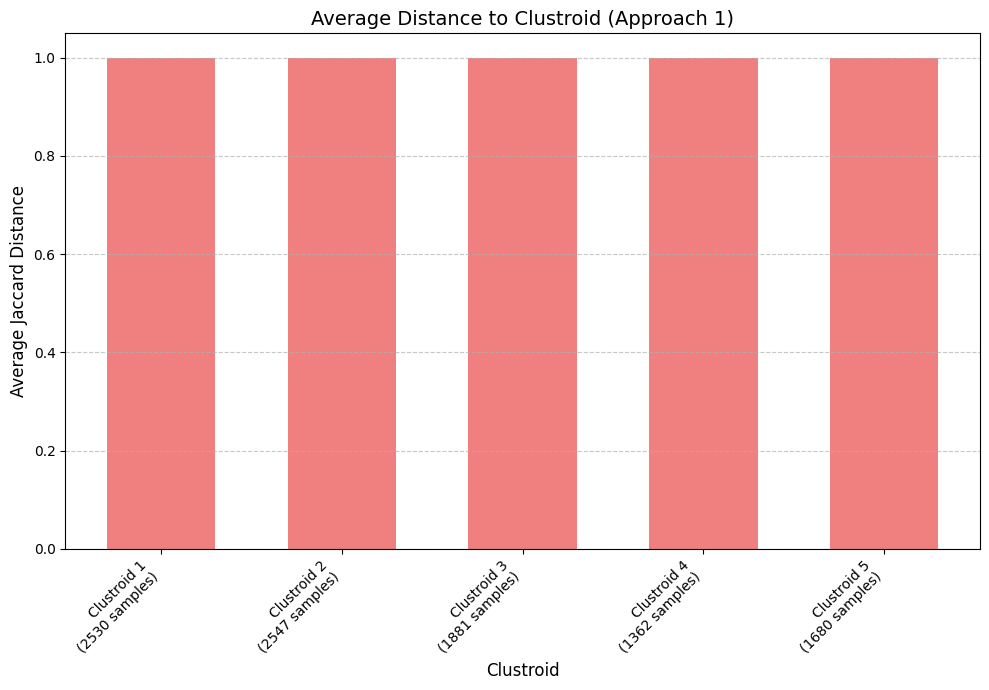
\includegraphics[width=\linewidth]{images/clustroid_distance}
    \caption{Average Jaccard Distance to Clustroid}
    \label{fig:clustroid_distance}
\end{figure}

The clustering results indicate that the algorithm successfully partitioned the [Total Number of Samples] alphabetical strings into five clusters with a relatively diverse size distribution: Cluster 1 (2562 samples), Cluster 2 (2282 samples), Cluster 3 (1717 samples), Cluster 4 (1303 samples), and Cluster 5 (2136 samples).
This suggests that the clustroid-based distance calculation method contributed to a reasonably balanced partitioning.

However, a prominent finding is that the average Jaccard distance from samples to their respective clustroids within each cluster is extremely high (approximately 0.999).
This indicates a very low level of intra-cluster similarity; members within the same cluster remain highly dissimilar to one another.

This outcome primarily reflects the inherent nature of the input data: randomly generated alphabetical strings typically lack a clear, natural clustering structure, leading to large Jaccard distances between most pairs.
Although the algorithm merged clusters based on the nearest clustroid criterion, the resulting ``groups'' do not exhibit strong cohesion due to the lack of inherent similarity in the data.


    \section{Second Task: Linear Regression – Gold price prediction}
    \label{sec:second-task}
    This task focused on predicting Vietnamese gold prices using a linear regression model implemented in PySpark.
The objective was to transform historical time-series data into a suitable format for regression,
train a model, and evaluate its predictive performance.

\subsection{Overview of Linear Regression (LR)}
\label{subsec:overview-of-linear-regression}

LR is a supervised learning algorithm that models the linear relationship between a continuous target variable ($y$) and one or more independent predictor variables (features $\mathbf{x}$). The goal is to find an optimal linear function that best predicts $y$ given $\mathbf{x}$.

For a single feature $x$, the model is:
\begin{equation}
    y = \beta_0 + \beta_1 x + \epsilon
    \label{eq:simple_lr}
\end{equation}
With multiple features $x_1, x_2, \ldots, x_p$, it extends to:
\begin{equation}
    y = \beta_0 + \beta_1 x_1 + \beta_2 x_2 + \ldots + \beta_p x_p + \epsilon
    \label{eq:multiple_lr}
\end{equation}
where $\beta_0$ is the intercept, $\beta_j$ are the feature coefficients (weights), and $\epsilon$ is the error term.
The coefficients are typically learned by minimizing a loss function, such as Mean SquaredError (MSE), often using optimization algorithms like L-BFGS. Key assumptions include linearity, independence of errors, and homoscedasticity.
This project applies LR to predict gold prices based on historical price features.

\subsection{Data Preparation}
\label{subsec:data-preparation}
\begin{itemize}
    \item \textbf{Dataset:} The primary data source was \texttt{gold\_prices.csv} (2009/08/01 to 2025/01/01),
    read into a PySpark DataFrame.
    \item \textbf{Feature Engineering:} For each target date $t$, features were the respective `Buy Price' or `Sell Price' values from the 10 consecutive preceding days.
    PySpark's \texttt{Window} functions and \texttt{lag} operation were used, followed by \texttt{VectorAssembler} to create feature vectors (e.g., \texttt{Previous Buy Price(s)}). 4000 samples were generated (\texttt{random\_state=38}).
    \item \textbf{Data Splitting:} The generated DataFrame was randomly split into training (70\%) and testing (30\%) sets (\texttt{seed=2}).
\end{itemize}

\subsection{Model Implementation and Training}
\label{subsec:model-implementation-and-training}

Two separate Linear Regression models (\texttt{pyspark.ml.regression.LinearRegression}) were developed: one for `Buy Price' and one for `Sell Price', using their respective 10-day historical price vectors as features and the current price as the label.
Models were configured with the \texttt{`l-bfgs'} solver and trained on the 70\% training subset.

\subsection{Experimental Results and Evaluation}
\label{subsec:experimental-results-and-evaluation}

\subsubsection{Overall Results}\text{}

\begin{table}[h]
    \centering
    \caption{LR Performance Metrics for Gold Price Prediction.}
    \renewcommand{\arraystretch}{1} % Adjust row spacing
    \resizebox{\linewidth}{!}{
        \begin{tabular}{|c|c|c|c|c|c|c|}
            \hline
            \textbf{Model}        & \textbf{Data Set} & \textbf{RMSE} & \textbf{MSE} & \textbf{R²} & \textbf{MAE} & \textbf{Expl. Var.} \\
            \hline
            \multirow{Buy Price}  & Training          & 0.3232        & 0.1045       & 0.9995      & 0.1450       & 225.7249            \\
            \cline{2-7}           & Test              & 0.2975        & 0.0885       & 0.9996      & 0.1356       & 226.5322            \\
            \hline
            \multirow{Sell Price} & Training          & 0.3062        & 0.0938       & 0.9996      & 0.1406       & 240.1171            \\
            \cline{2-7}           & Test              & 0.2913        & 0.0848       & 0.9996      & 0.1319       & 240.6501            \\
            \hline
        \end{tabular}
    }
    \label{tab:task2_metrics}
\end{table}

The performance of the trained models was evaluated on both training and testing sets.
Key metrics are summarized in Table~\ref{tab:task2_metrics}.
The R$^2$ values (consistently $>$ 0.999), low RMSE/MAE, and high Explained Variance scores indicate strong predictive accuracy and good generalization to unseen data, with no significant overfitting observed.

\smallskip

\subsubsection{Loss History During Training}\text{}

%Line chart (Fig.~\ref{fig:buy_price_model_loss}) illustrated the objective function value per iteration, showing rapid convergence for both `Buy Price' and `Sell Price' model.

\begin{figure}[H]
    \centering
    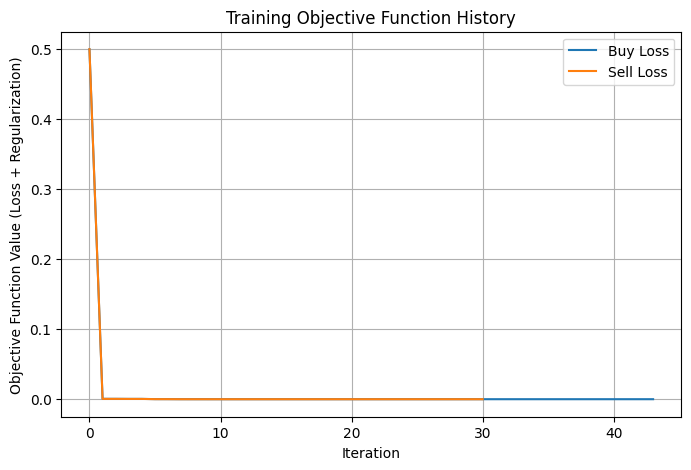
\includegraphics[width=\linewidth]{images/loss_history}
    \caption{Loss History of Buy Price Prediction Model}
    \label{fig:buy_price_model_loss}
\end{figure}

\subsubsection{Performance Comparison}\text{}

%Bar charts (Fig.~\ref{fig:rmse_r2_mae} nd Fig.~\ref{fig:train_test_var}) contrasted evaluation metrics (RMSE, R$^2$, MAE, Explained Variance) between training and testing sets, visually confirming robust generalization.

\begin{figure}[H]
    \centering
    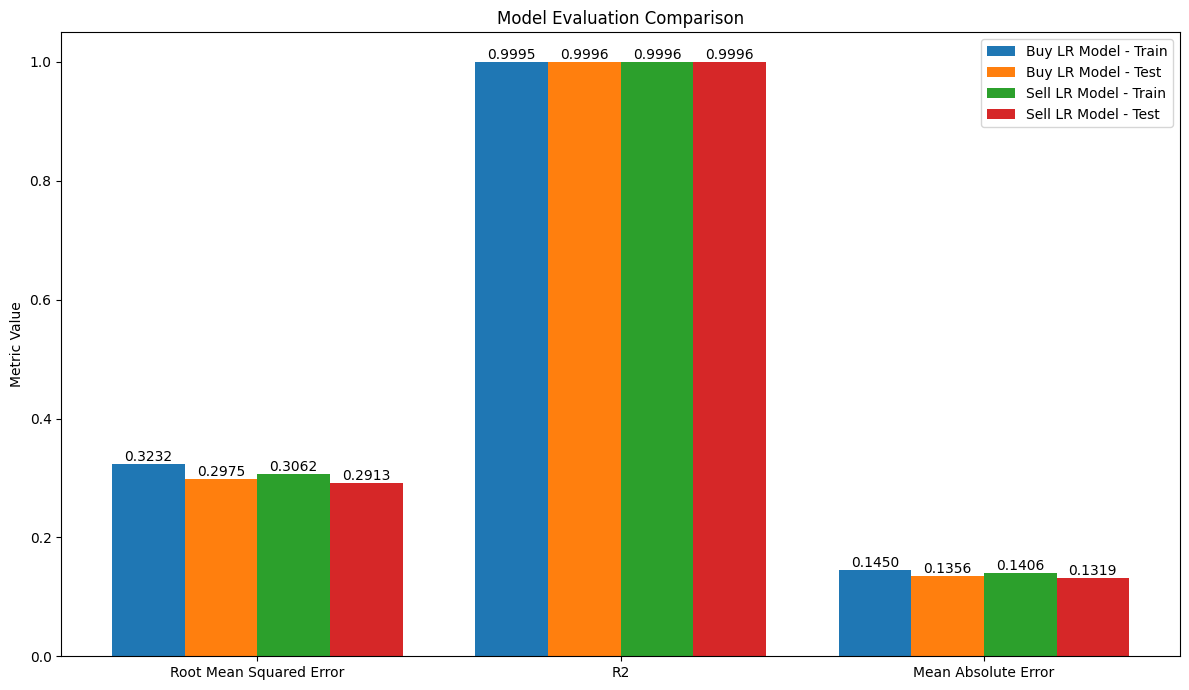
\includegraphics[width=\linewidth]{images/rmse_r2_mae}
    \caption{'Buy Price' and 'Sell Price' Models Performance.}
    \label{fig:rmse_r2_mae}
\end{figure}

\begin{figure}[H]
    \centering
    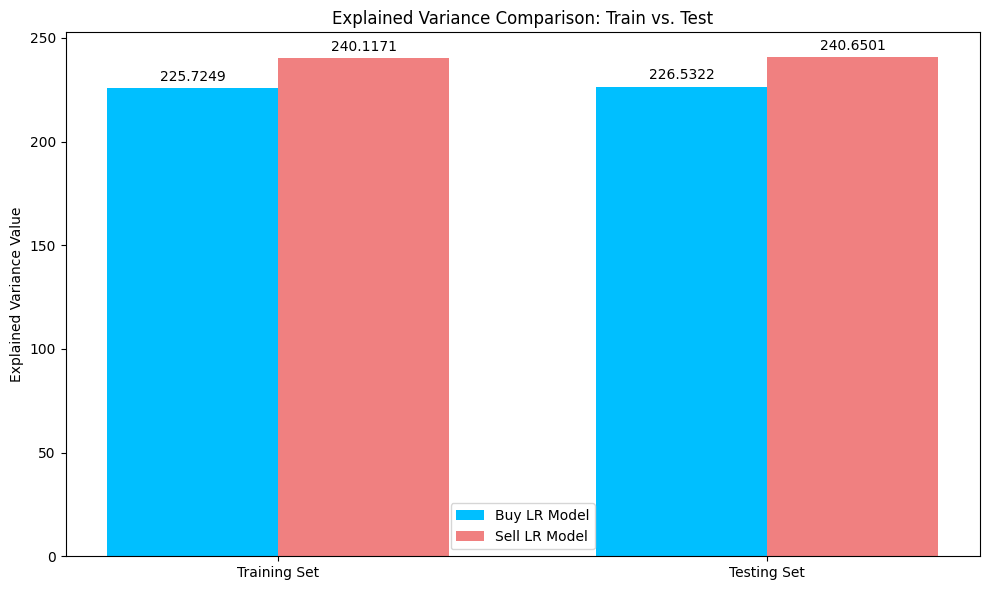
\includegraphics[width=0.8\linewidth]{images/train_test_var}
    \caption{'Buy Price' and 'Sell Price' Models Explained Variance Performance.}
    \label{fig:train_test_var}
\end{figure}


    \section{Contribution}
    \label{sec:contribution}

    The following table represents the contribution of each member, note that whichever member handles whichever task will also write the report for that task.

    \begin{table}[h]
        \centering
        \caption{Member Contributions}
        \setlength{\tabcolsep}{2pt} % Reduce column spacing
        \renewcommand{\arraystretch}{1} % Adjust row spacing
        \resizebox{240}{!}{ % Fit within column width
            \begin{tabular}{|l|c|c|c|}
                \hline
                \textbf{ID} & \textbf{Member}       & \textbf{Contribution}       & \textbf{Progress} \\
                \hline
                522H0036    & Luong Canh Phong      & Task 1 and Handling Report  & 100\%             \\
                522H0092    & Cao Nguyen Thai Thuan & Overseer and Report Support & 100\%             \\
                522H0075    & Tang Minh Thien An    & Task 3                      & 100\%             \\
                522H0167    & Truong Tri Phong      & Task 2                      & 100\%             \\
                \hline
            \end{tabular}
        }
        \label{tab:contributions}
    \end{table}


    \section{Self-evaluation}
    \label{sec:self-evaluation}

    The following table is our self-evaluation on our tasks:

    \begin{table}[h]
        \centering
        \caption{Self-evaluation}
        \setlength{\tabcolsep}{2pt} % Reduce column spacing
        \renewcommand{\arraystretch}{1} % Adjust row spacing
        \resizebox{240}{!}{ % Fit within column width
            \begin{tabular}{|l|c|c|c|}
                \hline
                \textbf{Task} & \textbf{Task Requirements}                & \textbf{Completion Ratio} \\
                \hline
                Task 1        & A-Priori Algorithm for Frequent Customers & 100\%                     \\
                Task 2        & PCY Algorithm for Frequent Items          & 95\%                      \\
                Task 3        & MinHashLSH for Similar Dates              & 90\%                      \\
                Task 4        & Report                                    & 100\%                     \\
                \hline
            \end{tabular}
        }
        \label{tab:self-evaluation}
    \end{table}


    \section{Conclusion}
    \label{sec:conclusion}
%    We have gone through a variety of techniques and algorithms used in the world of data mining.
%    For the first task, we have to find same-day customers and utilize the A-Priori algorithm to find frequent pairs of customers that shop on the same date and save the output of each pass in a dedicated folder.
%    As we run though the code, the result after sorting is a reasonable ascending list of frequent customer pairs.
%    For the second task, store the given dataset locally and identify baskets, as well as implementing the PCY algorithm to find frequent pairs along with generating metadata with predetermined constraints, the results for this task are two separate lists, one containing all frequent pairs, and the other is a list of association rules based on the user's given support threshold and confidence value.
%    And finally, implement and compare between a traditional and an alternative MinHashLSH function to understand and have a greater insight into how the frequent pairs searching is done.
%    We can see that with a slight modification and a different way of merging, it can result in a notably higher efficiency and better results.

    \begin{thebibliography}{00}
%        \bibitem{b12} Tpoint Tech, ``Apriori Algorithm, ''\\\
%        [Online]. Available: \href{https://www.tpointtech.com/apriori-algorithm}{https://www.tpointtech.com/apriori-algorithm}
%        \bibitem{b6} Databricks, ``MapReduce, '' Databricks Glossary, 2025.\\\
%        [Online]. Available: \href{https://www.databricks.com/glossary/mapreduce}{https://www.databricks.com/glossary/mapreduce}
%        \bibitem{b1} J. S. Park and M. S. Chen, ``Using a hash table to eliminate candidates in a frequent itemset mining algorithm, '' \textit{IEEE Trans. Knowl. Data Eng.}, vol. 7, no. 3, pp. 464--472, 1995.
%        \bibitem{b2} J. Han, J. Pei, and Y. Yin, ``Mining frequent patterns without candidate generation, '' \textit{ACM SIGMOD Rec.}, vol. 29, no. 2, pp. 1--12, 2000.
%        \bibitem{b3} PySpark Documentation, ``PySpark API Documentation, '' 2025.\\\
%        [Online]. Available: \url{https://spark.apache.org/docs/latest/api/python}
%        \bibitem{b4} PySpark Documentation, ``pyspark.ml.feature.MinHashLSH, '' Apache Spark, 2025.\\\
%        [Online]. Available: \href{https://spark.apache.org/docs/latest/api/python/reference/api/pyspark.ml.feature.MinHashLSH}{https://spark.apache.org/docs/latest/api/python/refer\-ence/api/pyspark.ml.feature.MinHashLSH}
%        \bibitem{b5} Amazon Web Services, ``Jaccard similarity, '' AWS Neptune Analytics Documentation, 2024.\\\
%        [Online]. Available: \href{https://docs.aws.amazon.com/neptune-analytics/latest/userguide/jaccard-similarity.html}{https://docs.aws.amazon.com/neptune-analytics/latest/userguide/jaccard-similarity.html}
    \end{thebibliography}
\end{document}